\documentclass{ieeeaccess}
\usepackage{cite}
\usepackage{amsmath,amssymb,amsfonts}
\usepackage{graphicx}
\usepackage{textcomp}
\usepackage{bm}
\usepackage{url}
\makeatletter
\AtBeginDocument{\DeclareMathVersion{bold}
\SetSymbolFont{operators}{bold}{T1}{times}{b}{n}
\SetSymbolFont{NewLetters}{bold}{T1}{times}{b}{it}
\SetMathAlphabet{\mathrm}{bold}{T1}{times}{b}{n}
\SetMathAlphabet{\mathit}{bold}{T1}{times}{b}{it}
\SetMathAlphabet{\mathbf}{bold}{T1}{times}{b}{n}
\SetMathAlphabet{\mathtt}{bold}{OT1}{pcr}{b}{n}
\SetSymbolFont{symbols}{bold}{OMS}{cmsy}{b}{n}
\renewcommand\boldmath{\@nomath\boldmath\mathversion{bold}}}
\makeatother

\begin{document}
\history{Date of publication xxxx 00, 0000, date of current version xxxx 00, 0000.}
\doi{10.1109/ACCESS.2024.0429000}

\title{Does a Quantum Reservoir Computing Advantage in Volatility Forecasting Survive Honest Evaluation? A Pre-Registered Audit}

\author{\uppercase{Sandanayakage Janindu Indira Sandanayaka}\authorrefmark{1},
\uppercase{Maninda Edirisooriya}\authorrefmark{1}, AND \uppercase{Achala Aponso}\authorrefmark{1}}

\address[1]{Informatics Institute of Technology, Colombo, Sri Lanka, in collaboration with the University of Westminster, London, U.K. (e-mail: janindu.20232270@iit.ac.lk)}

\tfootnote{This work did not receive any specific funding.}

\markboth
{S. J. I. Sandanayaka \headeretal: Auditing a Quantum Reservoir Advantage in Volatility Forecasting}
{S. J. I. Sandanayaka \headeretal: Auditing a Quantum Reservoir Advantage in Volatility Forecasting}

\corresp{Corresponding author: S. J. I. Sandanayaka (e-mail: janindu.20232270@iit.ac.lk).}

\begin{abstract}
Claims that quantum machine learning forecasts financial time series better than classical methods are appearing quickly, but they are rarely re-examined. We audit one such claim: a published study reporting that a ten-qubit quantum reservoir computer forecasts monthly realized volatility of the United States stock market better than linear and neural benchmarks. Using the authors' public data and couplings, our independent implementation reproduces their published forecasts to within one part in a million. We then test the claim under a protocol registered before each analysis. On the registered primary loss, selecting the reservoir instance on a validation window instead of the test period removes statistical significance against a standard heterogeneous autoregressive benchmark, and a tuned classical echo state network of the same size matches the quantum model. The published reservoir instances rank fifth and seventh of one hundred on test error, and greedy forward feature selection scored on the test period reproduces both published input sets exactly, whereas selection on a validation window does not and loses the edge. We prove that every readout is a multilinear trigonometric function of the inputs, and a second-order trigonometric model reproduces the readouts with holdout fit of essentially one. A power analysis shows the 245-month sample cannot reliably detect gains below about fifteen percent. Transferred to eight commodity futures, the design shows no advantage in any market. On IBM quantum hardware, noise removes the remaining forecasting value. We release a reusable audit protocol for quantum forecasting claims.
\end{abstract}

\begin{keywords}
Data snooping, forecast evaluation, quantum computing, quantum machine learning, quantum reservoir computing, realized volatility, reproducibility.
\end{keywords}

\titlepgskip=-21pt

\maketitle

% ===========================================================================
\section{Introduction}
\label{sec:introduction}
\PARstart{Q}{uantum} machine learning (QML) is increasingly applied to financial forecasting, and several recent studies report that quantum models outperform classical ones. Such claims matter beyond academia: they inform investment in quantum hardware and in quantum software for finance. Yet three features of the field make advantage claims fragile. First, the classical baselines in QML papers are often weak or untuned, a problem documented for QML in general by Bowles \emph{et al.}~\cite{bowles2024}. Second, many quantum models used on near-term hardware can be simulated, or even replaced, by classical models built from the same Fourier spectrum~\cite{schuld2021,schreiber2023,sweke2025}. Third, financial forecasting comparisons are vulnerable to data snooping: when many model variants are tried and the best one is reported on the same test sample, apparent skill is biased upward~\cite{white2000,hansen2005,bailey2014}. Leakage of this kind is a known source of irreproducible results across machine-learning-based science~\cite{kapoor2023}.

Large benchmarks have shown that quantum models struggle to beat classical models of comparable complexity on time series~\cite{fellner2026}, and attribution audits in other domains have begun to separate quantum from classical sources of performance~\cite{gillani2026}. What is missing is a direct re-examination of a specific, published quantum advantage claim in financial forecasting, using the authors' own data, under a protocol fixed in advance.

Audits of this kind are common in empirical finance and medicine, where a published result is re-run on the original data before it is built upon, but they are rare in QML. Most QML evaluations either propose a new model or benchmark many models on new data. Neither shows whether a specific published advantage was real, because neither repeats the published analysis and then changes one decision at a time to see which decision the advantage depends on.

We provide such a re-examination for the study of Li, Mukhopadhyay, Bayat, and Habibnia~\cite{li2026}, published in \emph{Physical Review Research} in 2026. It reports that quantum reservoir computing (QRC) forecasts monthly realized volatility (RV) of the S\&P 500 better than autoregressive, heterogeneous autoregressive (HAR), long short-term memory, and classical reservoir benchmarks. The study is well suited to an audit: its code, data, and the 100 random coupling matrices are public, and the model is small enough (ten qubits) to simulate exactly.

Our contributions are as follows.
\begin{enumerate}
\item \textbf{Exact reproduction.} An independent implementation reproduces the published one-step forecasts to within $1.2\times10^{-6}$ (Section~\ref{sec:res-repro}).
\item \textbf{Selection audit.} Selecting the reservoir on a validation window removes significance against a standard HAR model and against data-snooping-robust tests. The published reservoir instances are in the top decile of the test-error distribution, and test-scored forward selection reproduces both published feature lists exactly (Sections~\ref{sec:res-select} and~\ref{sec:res-features}).
\item \textbf{Matched classical controls.} Size-matched classical reservoirs, random-feature models, and a trigonometric surrogate are not significantly worse than the quantum model; the only control it beats consistently is its own uncoupled version (Section~\ref{sec:res-controls}).
\item \textbf{An exact classical description.} We prove that every readout is a multilinear trigonometric function of the inputs and show that a second-order truncation reproduces the readouts on the data (Section~\ref{sec:res-surrogate}, Appendix~\ref{app:proof}).
\item \textbf{Power, transfer, and hardware.} We quantify the smallest gain the published design can detect, test the design on eight commodity futures, and execute the reservoir circuit on an IBM quantum processor with a readout trained on hardware outputs (Sections~\ref{sec:res-power}--\ref{sec:res-hw}).
\end{enumerate}

Tests 2 to 8 were registered in frozen, hashed files before they were run, after the reproduction (Test 1) had been completed; one post-hoc change is disclosed (Appendix~\ref{app:deviations}). We stress what this audit does and does not show. It shows that the published evidence does not establish a quantum advantage. It does not show that the authors acted improperly: their paper does not state which sample scored the feature selection, and we describe the published choices only as consistent with, not proof of, test-period selection. Nor does it show that quantum reservoirs cannot help on other problems.

% ===========================================================================
\section{Related Work}
\label{sec:related}

\subsection{Quantum Reservoir Computing}
Reservoir computing trains only a linear readout on the states of a fixed dynamical system; the echo state network (ESN) is its standard classical form~\cite{jaeger2001}. QRC replaces the classical reservoir with a quantum system whose measured observables serve as features~\cite{fujii2017,mujal2021}. Finite-dimensional quantum reservoirs are state-affine systems, a class already studied in classical reservoir computing~\cite{martinezpena2023}. Because training reduces to ridge regression, QRC avoids the barren-plateau training problems of variational circuits, which makes it attractive for near-term hardware. Its expressive power is, however, limited by how data are encoded. For angle encoding, the model is a Fourier series in the inputs whose frequencies are set by the encoding~\cite{schuld2021}.

\subsection{Classical Surrogates and Dequantization}
Schreiber, Eisert, and Meyer showed that many quantum learning models admit efficient classical surrogates built from their Fourier spectrum~\cite{schreiber2023}. Sweke \emph{et al.} characterized when random Fourier features~\cite{rahimi2007} can and cannot dequantize such models~\cite{sweke2025}, and Hernicht \emph{et al.} made surrogate construction scale to a real energy-forecasting task~\cite{hernicht2026}. These works establish surrogates as a theoretical and engineering tool. We use an exact surrogate as an \emph{audit control} for a published claim.

\subsection{Quantum Machine Learning for Finance and Time Series}
Fellner \emph{et al.} benchmarked variational QML on 27 time-series tasks and found that quantum models struggle to match simple classical counterparts of comparable complexity~\cite{fellner2026}. In finance, Tudisco \emph{et al.} evaluated variational circuits for fraud detection in this journal~\cite{tudisco2024}. Gillani \emph{et al.} proposed a quantum-attribution audit for network intrusion detection, with parameter-matched classical controls and a random-feature kernel; they found tuned classical models matched or exceeded the quantum ones, although the quantum kernel outranked its direct random-feature surrogate~\cite{gillani2026}. Pandey showed that reported advantages of quantum reservoirs on synthetic forecasting tasks vanish once classical baselines receive the same size and tuning budget~\cite{pandey2026}. In finance, Shen found that a quantum kernel for stock returns appears dominant only on a universe screened with full-sample information~\cite{shen2026}; Islam showed, for attack detection, that evaluation choices can reverse conclusions with the models held fixed~\cite{islam2026}; and Maheshwari \emph{et al.} found no edge for quantum recurrent models on a financial series once matched controls and naive baselines were included~\cite{maheshwari2026}. We did not find a study that re-runs a named, published QML financial forecasting claim, on the authors' own data, against exact surrogates and size-matched controls under pre-registered protocols.

\subsection{Forecast Evaluation and Data Snooping}
RV is the standard nonparametric volatility measure~\cite{andersen2003}, and the HAR model is a strong, simple benchmark for it~\cite{corsi2009}. Forecast comparison uses the Diebold--Mariano (DM) test~\cite{diebold1995} with heteroskedasticity- and autocorrelation-consistent variance~\cite{newey1987}. When many models are compared, White's reality check~\cite{white2000}, Hansen's test for superior predictive ability (SPA)~\cite{hansen2005}, and the model confidence set (MCS)~\cite{hansen2011} control for data snooping. For volatility, squared error on log RV and the quasi-likelihood (QLIKE) loss are both used; QLIKE is robust to noise in the volatility proxy~\cite{patton2011}. Bailey \emph{et al.} showed how selecting among many backtests inflates out-of-sample claims~\cite{bailey2014}.

% ===========================================================================
\section{The Audited Study}
\label{sec:study}
Li \emph{et al.}~\cite{li2026} forecast monthly log RV of the S\&P 500 from February 1950 to December 2017, aligning their sample with an earlier neural-network study, together with macroeconomic and financial predictors of the Welch--Goyal type~\cite{welch2008}: the dividend--price ratio (DP), earnings--price ratio (EP), market excess return (MKT), size and value factors (SMB, HML), Treasury bill rate (TB), default spread (DEF), industrial production growth (IP), inflation (INF), short-term reversal (STR), and quarterly and annual averages of RV (RV$_q$, RV$_a$).

\subsection{Reservoir}
The reservoir has ten qubits with Hamiltonian
\begin{equation}
H=\sum_{i<j} J_{ij}\,X_iX_j+\sum_{i} Z_i,
\label{eq:ham}
\end{equation}
where $X_i$ and $Z_i$ are Pauli operators on qubit $i$ and the couplings $J_{ij}$ are drawn at random. Seven qubits are inputs and three are hidden. To forecast month $t$, the hidden qubits start in $|000\rangle$. For each lag $k=3,2,1$, the seven input qubits are freshly prepared as $R_Y(\pi x_{t-k,v})|0\rangle$ for input $v$, joined with the hidden qubits, and evolved for unit time by $e^{-iH}$; between lags the input qubits are discarded. The features are the expectation values $\langle Z_q\rangle$ of all ten qubits after the last evolution (QR1, ten features). QR2 additionally reads the qubits halfway through the last evolution (twenty features). Inputs are min--max scaled to fixed ranges.

\subsection{Readout and Evaluation}
A ridge regression without intercept ($\lambda=10^{-8}$) maps features to scaled log RV. It is re-estimated on a rolling window of 571 months, producing 245 one-step forecasts from August 1997 to December 2017. The paper evaluates 100 random coupling instances and states that it reports ``the best-performing quantum reservoir'', arguing that this is fair because the best long short-term memory configuration is also reported~\cite{li2026}. QR1 and QR2 each use seven inputs chosen by ``wrapper-based forward selection''; the sample used to score that selection is not stated.

% ===========================================================================
\section{Audit Protocol}
\label{sec:protocol}

\subsection{Pre-Registration}
Before each block of analyses we froze a JSON file stating the data, models, losses, decision rules, and scripts, and recorded its SHA-256 hash; the analysis scripts refuse to run if the file changes. Four registrations cover Tests 2--3, Test 7, Tests 4--6, and Test 8. Each states what was known when it was frozen. One change was made after results were seen and is reported as a dated addendum (Appendix~\ref{app:deviations}). Table~\ref{tab:tests} lists the tests, the decision rule fixed for each, and the outcome.

\begin{table*}[t]
\caption{\textbf{The registered tests and their outcomes}}
\label{tab:tests}
\setlength{\tabcolsep}{3pt}
\begin{tabular}{|l|p{120pt}|p{170pt}|p{150pt}|}
\hline
Test & Question & Registered rule & Outcome\\
\hline
1 & Does our implementation reproduce the published forecasts? & none; run before the first registration & reproduced, $1.2\times10^{-6}$\\
2 & Does the edge survive validation selection of the instance? & joint rule with Test 3: SPA must reject against both AR(3) and HAR & SPA rejects against AR(3) only\\
3 & Does it beat size-matched classical controls? & lower loss than all seven controls, Holm $p$ below 0.05, primary loss & not met; only QR-J0 (both) and RandTrig (QR1)\\
4 & Do scaling and feature selection matter? & descriptive; inputs called consistent with test-period selection if only test-scored selection reproduces them & scaling under 2\%; test-scored selection reproduces the published inputs\\
5 & Is the readout a trigonometric function of the inputs? & descriptive; Trig2 called an almost exact surrogate if median holdout $R^2$ exceeds 0.99 & residual $\le4\times10^{-15}$; order-two $R^2$ 1.000\\
6 & What gain can the design detect? & descriptive; minimum MSE reduction for 80\% power & 15--16\% (one test), 19--20\% (Holm)\\
7 & Does the design transfer to commodities? & quantum edge in at least five of eight assets & edge in 0 of 8 for both designs\\
8 & What happens on hardware? & descriptive; hardware reproduces the simulator if equivalent to the noiseless circuit & not equivalent; significantly worse than all three references\\
\hline
\end{tabular}
\end{table*}

\subsection{Independent Implementation}
We re-implemented the reservoir from the paper and the authors' code, and verified it against their published predictions (Test 1). For efficient exact simulation we keep the hidden-qubit density matrix in factored form $\rho_h=AA^\dagger$; because inputs are pure product states, each lag evolves at most $2^{3}$ vectors of dimension $2^{10}$, so 100 instances over 816 months run in minutes on a laptop CPU (Intel Core Ultra 9 185H). Simulations use Python 3.12 with NumPy 2.5 and SciPy 1.18, the bootstrap, SPA and MCS procedures use the arch package (version 8.0), and the hardware runs use Qiskit 2.6, Qiskit Aer 0.18 and Qiskit IBM Runtime 0.52.

\subsection{Selection Protocols}
We compare two ways of choosing among the 100 instances. \emph{Test-selected} picks the instance with the lowest test-period error, which reproduces the logic of reporting the best performer. \emph{Validation-selected} picks the instance with the lowest error on a validation window: the 120 months before the test period, each forecast from the preceding 451 months, using no test data.

\subsection{Classical Controls}
Each control is chosen on the same validation window and uses the same rolling ridge readout. For QR1 the controls have ten readout features and for QR2 twenty.
\begin{itemize}
\item \textbf{ESN:} a leaky echo state network run over the same three-lag window from a zero state, with a bias input. ESN-tuned selects leak rate, spectral radius, and input scale from a $3\times3\times3$ grid per instance, then the best of 100 instances.
\item \textbf{RandTrig:} random products of one to three terms $\cos(\pi x)$ or $\sin(\pi x)$ of the lagged inputs, mimicking the functional form of the reservoir (Section~\ref{sec:res-surrogate}).
\item \textbf{RFF:} random Fourier features~\cite{rahimi2007} with bandwidth chosen from $\{0.3,1,3\}$.
\item \textbf{Trig2:} the full second-order multilinear trigonometric basis (883 columns), with ridge penalty chosen on validation.
\item \textbf{QR-J0:} the quantum reservoir with all couplings set to zero, which removes entangling dynamics.
\item \textbf{AR(3)}, an autoregressive model of order three, and \textbf{HAR(1,3,12)}, with lags of one, three, and twelve months, both estimated by least squares on the same rolling window.
\end{itemize}

\subsection{Statistics}
The primary loss is squared error on log RV; the secondary loss is QLIKE on variance, $L(\sigma^2,h)=\sigma^2/h-\ln(\sigma^2/h)-1$ for realized variance $\sigma^2$ and forecast $h$~\cite{patton2011}. For each comparison we report the ratio of mean losses with a 95\% stationary-bootstrap interval (mean block length 6, 5000 resamples)~\cite{politis1994}, a two-sided DM test with Newey--West variance (lag 4)~\cite{diebold1995,newey1987}, and Holm-adjusted $p$-values within each table~\cite{holm1979}. A comparison is ``equivalent'' if its interval lies within $\pm3\%$. Over the 100 instances we report Hansen's SPA test against each benchmark (10\,000 resamples)~\cite{hansen2005} and a 95\% MCS~\cite{hansen2011}. The registered decision rule is that the published claim survives only if the validation-selected reservoir beats every control after Holm correction and the SPA test rejects for both AR(3) and HAR.

\subsection{Further Tests}
Test 4 changes the preprocessing: (a) min--max scaling on the first training window only, and (b) forward selection of seven of the 13 candidate inputs, scored on validation or on test. Test 5 checks the trigonometric structure of the readouts. Test 6 estimates the minimum detectable effect by simulation. Test 7 transfers the design to commodities. Test 8 runs the circuit on hardware. Details are given with each result.

% ===========================================================================
\section{Results}
\label{sec:results}

\subsection{Reproduction}
\label{sec:res-repro}
Our implementation reproduces the published QR1 and QR2 forecasts to within $1.2\times10^{-6}$ in log RV (Table~\ref{tab:repro}). AR(3) also reproduces. The paper's HAR benchmark has mean squared error (MSE) 0.1476, whereas a standard HAR(1,3,12) on the same data and window gives 0.1156. We use the standard HAR throughout, which is a stronger benchmark than the published one.

\begin{table}[t]
\caption{\textbf{Reproduction of the published results (245 test months)}}
\label{tab:repro}
\setlength{\tabcolsep}{4pt}
\begin{tabular}{|l|c|c|}
\hline
Model & Test MSE (log RV) & Note\\
\hline
QR1, published instance & 0.1051 & matches publication\\
QR2, published instance & 0.1038 & matches publication\\
AR(3) & 0.1181 & matches publication\\
HAR, as published & 0.1476 & from~\cite{li2026}\\
HAR(1,3,12), standard & 0.1156 & this work\\
\hline
\multicolumn{3}{p{230pt}}{Maximum absolute difference from the published QR forecasts: $1.2\times10^{-6}$. The published QLIKE values (1.4428 and 1.4004) also reproduce.}\\
\end{tabular}
\end{table}

\subsection{Honest Selection}
\label{sec:res-select}
Fig.~\ref{fig:hist} shows the test MSE of all 100 instances. The published instances rank 5th (QR1) and 7th (QR2). They are not the best by test MSE, nor by either QLIKE variant (ranks 4 to 10), so the paper's selection criterion cannot be recovered from the public material. The validation-selected instances are number 51 for QR1 (MSE 0.1064) and 97 for QR2 (0.1073). Across the 100 instances the median test MSE is 0.1094 for QR1 (5th to 95th percentile 0.1051 to 0.1136) and 0.1095 for QR2 (0.1037 to 0.1156); the best instances, 90 and 44, reach 0.1032 and 0.1018. All 100 QR1 instances and 94 of the 100 QR2 instances have lower test MSE than HAR, and all have lower test MSE than AR(3).

Against HAR, the validation-selected reservoirs have loss ratios 0.920 [0.822, 1.021] for QR1 and 0.929 [0.846, 1.020] for QR2, with DM $p=0.135$ and $0.119$. Against AR(3) the ratios are 0.901 [0.801, 0.997] and 0.909 [0.822, 0.999] ($p=0.061$ and $0.055$). Over the 100 instances, the SPA test rejects against AR(3) ($p=0.040$ and $0.024$) but not against HAR ($p=0.089$ and $0.059$). The reservoir family therefore forecasts somewhat better than the benchmarks in point terms, and every QR1 instance has lower test MSE than HAR, but the improvement over a standard HAR is not statistically established once the selection is honest. Note that all 100 instances use the published input lists, which Section~\ref{sec:res-features} links to the test period.

The paper's fairness argument, that the best quantum and best classical configurations are both reported, can be tested directly. When both the quantum reservoir and the ESN are chosen as the best of 100 on the test period, their loss ratio is 0.996 [0.897, 1.098] for QR1 and 1.020 [0.942, 1.106] for QR2. Under symmetric selection, the quantum reservoir and a classical reservoir of the same size are indistinguishable. The same holds when both are chosen on the validation window (ratios 1.023 [0.924, 1.131] and 1.011 [0.934, 1.090]).

\begin{figure*}[t]
\centering
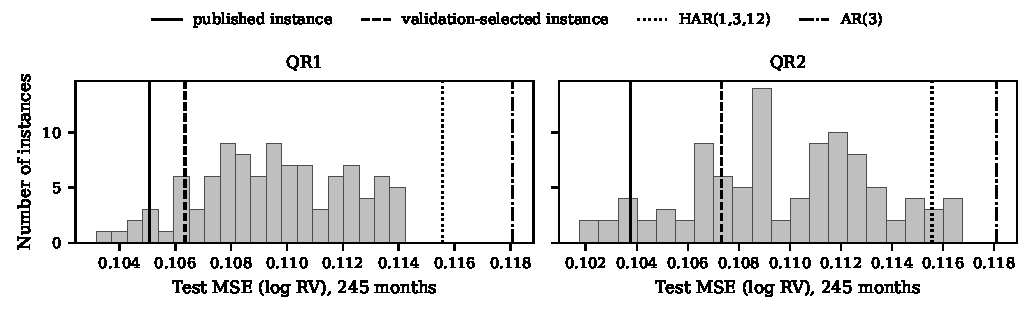
\includegraphics[width=\textwidth]{figs/sanda1.pdf}
\caption{Test MSE of the 100 random reservoir instances on the authors' data and window, with the published instance, the instance selected on the validation window, and two linear benchmarks. The published instances rank 5th (QR1) and 7th (QR2) of 100.}
\label{fig:hist}
\end{figure*}

\subsection{Size-Matched Classical Controls}
\label{sec:res-controls}
Table~\ref{tab:controls} compares the validation-selected reservoir with all controls. After Holm correction it is significantly better only than its uncoupled version QR-J0 (both designs) and, for QR1, the RandTrig control. It is not significantly better than the tuned ESN, RFF, Trig2, AR(3), or HAR. For QR2 the tuned ESN has the lower mean loss (ratio 1.014) and is the top-ranked model in the MCS; the quantum reservoir is in the MCS with $p=0.656$. For QR1 the quantum reservoir is top-ranked, but the MCS also retains the tuned ESN, RFF, Trig2, AR(3), and HAR. The registered decision rule therefore rejects the claim for both designs. The coupled reservoir does beat the uncoupled one, so the Hamiltonian dynamics matter, but a classical reservoir of the same size reproduces their benefit.

The 95\% MCS gives the same picture. Under squared error it removes only the uncoupled reservoir QR-J0, for both designs; the validation-selected reservoir, HAR, AR(3), Trig2, ESN-tuned, RandTrig and RFF remain in the set together (MCS $p\geq0.10$ for every retained control with QR1, $p\geq0.12$ with QR2). For QR2 the best-ranked model is ESN-tuned, not the reservoir (MCS $p$ of the reservoir 0.66). Under QLIKE the set for QR1 also excludes AR(3) ($p=0.04$) but keeps HAR ($p=0.11$), and for QR2 it keeps all eight models.

\begin{table}[t]
\caption{\textbf{Validation-selected reservoir versus controls, primary loss}}
\label{tab:controls}
\setlength{\tabcolsep}{2.5pt}
\begin{tabular}{|l|c|c|c|c|}
\hline
& \multicolumn{2}{c|}{QR1 (10 features)} & \multicolumn{2}{c|}{QR2 (20 features)}\\
Control & Ratio [95\% CI] & $p_\mathrm{Holm}$ & Ratio [95\% CI] & $p_\mathrm{Holm}$\\
\hline
ESN-tuned & 0.891 [0.740, 1.077] & 0.323 & 1.014 [0.951, 1.080] & 0.672\\
RandTrig$^\mathrm{a}$ & 0.845 [0.752, 0.942] & 0.036 & 0.923 [0.780, 1.067] & 0.630\\
RFF$^\mathrm{a}$ & 0.893 [0.772, 1.021] & 0.323 & 0.865 [0.743, 0.996] & 0.245\\
Trig2 & 0.880 [0.777, 0.983] & 0.142 & 0.895 [0.787, 1.012] & 0.287\\
QR-J0 & 0.862 [0.783, 0.937] & 0.023 & 0.873 [0.802, 0.947] & 0.029\\
AR(3) & 0.901 [0.801, 0.997] & 0.245 & 0.909 [0.822, 0.999] & 0.274\\
HAR(1,3,12) & 0.920 [0.822, 1.021] & 0.323 & 0.929 [0.846, 1.020] & 0.358\\
\hline
\multicolumn{5}{p{240pt}}{Ratio $<1$ means the quantum reservoir has lower loss. $p_\mathrm{Holm}$: Diebold--Mariano, Holm over the seven rows. $^\mathrm{a}$With a constant column (addendum A1, Appendix~\ref{app:deviations}). Registered versions without it: RandTrig 0.828 and 0.931, RFF 0.670 and 0.905, none significant after Holm.}\\
\end{tabular}
\end{table}

\subsection{Secondary Loss}
\label{sec:res-qlike}
The registered decision used squared error on log RV, but QLIKE on variance was registered as the secondary loss, and the reservoir does better under it (Table~\ref{tab:qlike}). For QR1, the point ratios against every control lie between 0.75 and 0.85. In the two-comparison family of honest selection, QR1 is significantly better than both HAR (ratio 0.844 [0.714, 0.982], $p_\mathrm{Holm}=0.030$) and AR(3) (0.809, $p_\mathrm{Holm}=0.010$). After Holm correction over all seven controls, it remains significantly better than AR(3), RandTrig and QR-J0, but not than HAR, the tuned ESN, RFF or Trig2 ($p_\mathrm{Holm}$ 0.085 to 0.090), and the SPA test over the 100 instances does not reject against HAR ($p=0.069$). The MCS retains the tuned ESN, HAR, RFF and Trig2 with the reservoir. For QR2 the reservoir is significantly better only than QR-J0 under QLIKE, and the tuned ESN has almost the same loss (ratio 0.998).

QLIKE penalizes forecasts that understate variance more than forecasts that overstate it, unlike squared error on log RV, so the two losses can rank models differently. Two caveats apply. These results use the published input lists, which Section~\ref{sec:res-features} links to the test period, and we did not repeat the feature-selection test under QLIKE. And the registered rule required significance against every control, which QLIKE does not provide either. We therefore report the secondary loss as the most favorable evidence for the claim, not as a reversal of the decision.

\begin{table}[t]
\caption{\textbf{Validation-selected reservoir versus controls, QLIKE}}
\label{tab:qlike}
\setlength{\tabcolsep}{2.5pt}
\begin{tabular}{|l|c|c|c|c|}
\hline
& \multicolumn{2}{c|}{QR1 (10 features)} & \multicolumn{2}{c|}{QR2 (20 features)}\\
Control & Ratio [95\% CI] & $p_\mathrm{Holm}$ & Ratio [95\% CI] & $p_\mathrm{Holm}$\\
\hline
ESN-tuned & 0.804 [0.661, 1.035] & 0.090 & 0.998 [0.914, 1.087] & 0.965\\
RandTrig & 0.747 [0.636, 0.851] & 0.002 & 0.840 [0.665, 1.034] & 0.397\\
RFF & 0.806 [0.654, 0.962] & 0.085 & 0.870 [0.747, 0.999] & 0.204\\
Trig2 & 0.843 [0.757, 0.960] & 0.090 & 0.838 [0.704, 1.007] & 0.397\\
QR-J0 & 0.777 [0.671, 0.869] & 0.003 & 0.856 [0.750, 0.947] & 0.040\\
AR(3) & 0.809 [0.675, 0.938] & 0.025 & 0.877 [0.761, 0.986] & 0.164\\
HAR(1,3,12) & 0.844 [0.714, 0.982] & 0.090 & 0.916 [0.803, 1.022] & 0.397\\
\hline
\multicolumn{5}{p{240pt}}{QLIKE on variance; otherwise as Table~\ref{tab:controls}. SPA over the 100 instances: QR1 $p=0.021$ against AR(3) and $0.069$ against HAR; QR2 $0.116$ and $0.284$.}\\
\end{tabular}
\end{table}

\subsection{Preprocessing and Feature Selection}
\label{sec:res-features}
\emph{Scaling.} The published inputs are min--max scaled over the full sample, and some inputs reach their extremes only in the test period. Re-scaling on the first training window only raises the MSE of the published instances from 0.1051 to 0.1067 (QR1) and from 0.1038 to 0.1056 (QR2); ratios 1.015 and 1.018, not significant. This look-ahead is a genuine flaw but explains less than 2\% of the error. With train-only scaling, neither the published nor the validation-selected instance beats AR(3) or HAR on the primary loss after Holm correction. Under QLIKE, train-only scaling leaves the QR1 results unchanged (Table~\ref{tab:scaling}).

\begin{table}[t]
\caption{\textbf{Effect of train-only scaling}}
\label{tab:scaling}
\setlength{\tabcolsep}{3pt}
\begin{tabular}{|l|c|c|c|}
\hline
& \multicolumn{3}{c|}{Test MSE (log RV)}\\
Instance & Full-sample & Train-only & Ratio [95\% CI]\\
\hline
QR1, published & 0.1051 & 0.1067 & 1.015 [0.984, 1.047]\\
QR1, validation-selected & 0.1064 & 0.1081 & 1.016 [0.983, 1.051]\\
QR2, published & 0.1038 & 0.1056 & 1.018 [0.976, 1.059]\\
QR2, validation-selected$^\mathrm{a}$ & 0.1073 & 0.1079 & 1.005 [0.948, 1.068]\\
\hline
\multicolumn{4}{p{240pt}}{Ratio: train-only over full-sample scaling; none significant. Under train-only scaling, QR1 against HAR: published 0.923 [0.832, 1.016], validation-selected 0.935 [0.842, 1.037] on the primary loss; 0.841 and 0.842 under QLIKE ($p_\mathrm{Holm}=0.035$). $^\mathrm{a}$Instance 16 is selected under train-only scaling.}\\
\end{tabular}
\end{table}

\emph{Feature selection.} Table~\ref{tab:features} and Fig.~\ref{fig:fs} show forward selection of seven of the 13 candidate inputs, using the published instances. When each step is scored on test MSE, the procedure selects exactly the published input lists, in the published order, for both designs. When each step is scored on the validation window, it selects different inputs, and the resulting test MSE (0.1253 and 0.1127) is no better than HAR (0.1156); for QR1 it is worse than both HAR and AR(3). There are about $8.6\times10^{6}$ ordered choices of seven inputs from 13, and the test-scored search recovers both published sequences. We conclude, as the registration specified, that the published input lists are consistent with selection on the test period. This is not proof of how the authors selected them; the selection code is not in the public repository.

\begin{table}[t]
\caption{\textbf{Forward selection of seven inputs (published instances)}}
\label{tab:features}
\setlength{\tabcolsep}{3pt}
\begin{tabular}{|l|l|p{118pt}|c|}
\hline
Design & Scored on & Inputs in order of selection & Test MSE\\
\hline
QR1 & published & RV, MKT, DP, IP, RV$_q$, STR, DEF & 0.1051\\
QR1 & test & RV, MKT, DP, IP, RV$_q$, STR, DEF & 0.1051\\
QR1 & validation & RV, TB, SMB, IP, DP, STR, RV$_q$ & 0.1253\\
\hline
QR2 & published & RV, MKT, STR, RV$_q$, EP, INF, DEF & 0.1038\\
QR2 & test & RV, MKT, STR, RV$_q$, EP, INF, DEF & 0.1038\\
QR2 & validation & RV$_a$, RV, MKT, IP, TB, EP, DP & 0.1127\\
\hline
\multicolumn{4}{p{240pt}}{For reference, HAR(1,3,12) 0.1156 and AR(3) 0.1181.}\\
\end{tabular}
\end{table}

\begin{figure*}[t]
\centering
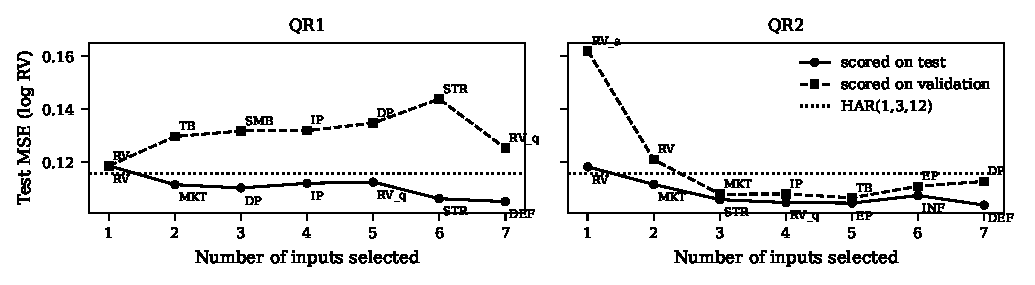
\includegraphics[width=\textwidth]{figs/sanda2.pdf}
\caption{Test MSE along the forward-selection path when each step is scored on the test period (solid) or on the validation window (dashed). Labels give the input added at each step. Test-scored selection reproduces the published input lists; validation-scored selection does not beat HAR.}
\label{fig:fs}
\end{figure*}

\subsection{An Exact Trigonometric Description}
\label{sec:res-surrogate}
\emph{Proposition.} Each readout $\langle Z_q\rangle$ of QR1 and QR2 is a multilinear function of the 21 triples $(1,\cos\pi x_{t-k,v},\sin\pi x_{t-k,v})$, $k\in\{1,2,3\}$, $v\in\{1,\dots,7\}$; that is, it lies in the span of products that contain at most one of $\cos\pi x_{t-k,v}$ or $\sin\pi x_{t-k,v}$ for each input.

The proof (Appendix~\ref{app:proof}) uses only the facts that each input value enters through exactly one freshly prepared qubit and that the reservoir is a linear map of each input's density matrix. The result holds for any couplings, so it covers all 100 instances, and it extends to any reservoir with this re-encoding structure.

Numerically, sweeping one input while holding the other 20 fixed fits $a+b\cos\pi x+c\sin\pi x$ to every readout with residual at most $1.1\times10^{-15}$ (QR1) and $4.0\times10^{-15}$ (QR2). The full span has $3^{21}$ terms, but low orders suffice on these data. On holdout windows drawn from the empirical input distribution, the order-one basis (43 columns) explains a median 98.9\% (QR1) and 99.4\% (QR2) of the variance of each readout, and the order-two basis (883 columns) explains 100.0\% (minimum over readouts 1.000). Under uniform inputs the order-two fit is lower in the worst case (minimum 0.954 and 0.958). On this problem, the reservoir is therefore, for practical purposes, a fixed low-order trigonometric feature map. The Trig2 control, which uses the whole order-two basis with a tuned ridge penalty, forecasts slightly worse than the reservoir (Table~\ref{tab:controls}), which is consistent with an 883-column regression on a 571-month window being harder to regularize than ten fixed features, not with the reservoir computing something outside the span.

\subsection{Statistical Power}
\label{sec:res-power}
How large a gain could the published design detect? We simulated competitors whose errors have the empirical correlation with HAR errors (0.91 for QR1, 0.90 for QR2) and a true MSE reduction $\delta$, resampled the HAR errors with the stationary bootstrap, and recorded how often a 5\% DM test detects the gain (2000 replications per $\delta$). Fig.~\ref{fig:power} and Table~\ref{tab:power} show the results. With 245 months, 80\% power requires a true reduction of about 15--16\% for a single test and 19--20\% when the comparison is the most significant of seven with Holm correction. The observed gains over HAR, 7--8\%, are about half of what the sample can reliably detect. With 120 months, as in our commodity transfer, the threshold rises to 19--27\%. Such designs can show that a model is clearly worse than a benchmark, but they cannot confirm realistic improvements. The registered grid (1, 2, 3, 5, 7.5, 10, 15, 20\%) gives the same conclusions as the finer grid in Fig.~\ref{fig:power}.

\begin{table}[t]
\caption{\textbf{Minimum MSE reduction over HAR detectable with 80\% power}}
\label{tab:power}
\setlength{\tabcolsep}{3pt}
\begin{tabular}{|l|c|c|c|c|}
\hline
Setting & Months & Single test & Holm, 1 of 7 & Observed ratio\\
\hline
Li \emph{et al.} data, QR1 & 245 & 15\% & 19\% & 0.920\\
Li \emph{et al.} data, QR2 & 245 & 16\% & 20\% & 0.929\\
Copper, QR1 & 120 & 19\% & 25\% & 1.108\\
Copper, QR2 & 120 & 21\% & 27\% & 1.057\\
\hline
\multicolumn{5}{p{240pt}}{Supplementary 1\%-step grid. Observed ratio: validation-selected reservoir over HAR.}\\
\end{tabular}
\end{table}

\begin{figure}[t]
\centering
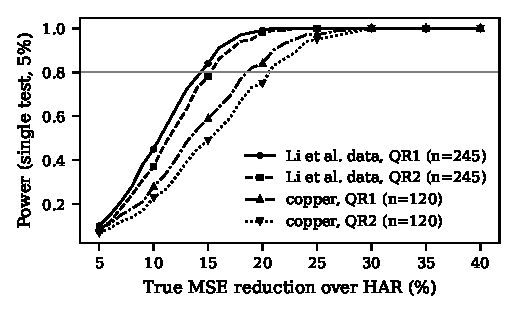
\includegraphics[width=\columnwidth]{figs/sanda4.pdf}
\caption{Simulated power of a 5\% Diebold--Mariano test to detect a true MSE reduction over HAR, for the published 245-month design and the 120-month copper transfer. The horizontal line marks 80\% power.}
\label{fig:power}
\end{figure}

\subsection{Where the Edge Comes From}
\label{sec:res-concentration}
The low power has a visible cause. Fig.~\ref{fig:cumloss} plots the running sum of the squared-error gain of each reservoir over HAR across the 245 test months. The curve climbs in a few jumps, in August 1998, September 2001, July 2002, August 2007, October 2008 and late 2014, and rises more slowly in between; in 2000 the reservoirs fall well behind HAR. Table~\ref{tab:concentration} quantifies this. The ten months in which a reservoir beats HAR by most supply 89\% to 123\% of its total gain; on the other 235 months its MSE ratio to HAR is between 0.986 and 1.023. The same holds for the classical models that also beat HAR: for the ESN controls the ten best months supply 75\% to 92\% of the gain. The concentration is therefore a property of this sample, not of the quantum reservoir, and it explains why one 245-month sample cannot separate models whose average errors differ by a few percent. This analysis was not registered and is descriptive.

\begin{table}[t]
\caption{\textbf{Concentration of the gain over HAR (Li \emph{et al.} data)}}
\label{tab:concentration}
\setlength{\tabcolsep}{3pt}
\begin{tabular}{|l|c|c|c|}
\hline
Model & Ratio to HAR & Top-10 share & Other 235 months\\
\hline
QR1, published & 0.909 & 103\% & 1.004\\
QR1, validation-selected & 0.920 & 122\% & 1.023\\
QR2, published & 0.898 & 89\% & 0.986\\
QR2, validation-selected & 0.929 & 123\% & 1.020\\
ESN, size of QR1 & 0.900 & 75\% & 0.967\\
ESN, size of QR2 & 0.918 & 89\% & 0.989\\
ESN-tuned, size of QR2 & 0.916 & 92\% & 0.992\\
\hline
\multicolumn{4}{p{240pt}}{Top-10 share: part of the total squared-error gain over HAR earned in the ten months with the largest gain; above 100\% means the other months together favor HAR. Other 235 months: MSE ratio to HAR without those ten months. Controls are validation-selected. Post hoc, descriptive.}\\
\end{tabular}
\end{table}

\begin{figure}[t]
\centering
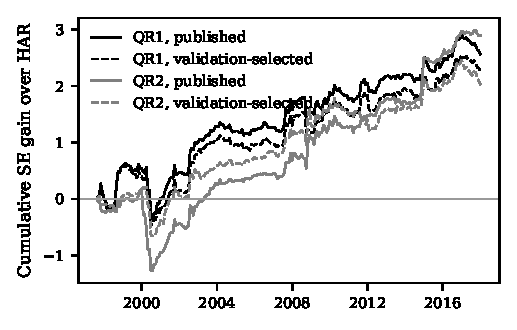
\includegraphics[width=\columnwidth]{figs/sanda6.pdf}
\caption{Cumulative squared-error gain of the quantum reservoirs over HAR across the 245 test months (August 1997 to December 2017), for the published and the validation-selected instances. Rises mean the reservoir beats HAR in that month.}
\label{fig:cumloss}
\end{figure}

\subsection{Transfer to Commodity Futures}
\label{sec:res-transfer}
We applied the exact published design, with the same 100 coupling matrices, to monthly RV of eight futures contracts: copper (HG), crude oil (CL), gold (GC), heating oil (HO), natural gas (NG), corn (ZC), soybeans (ZS), and wheat (ZW). RV is the square root of the sum of squared daily log returns in a month, from continuous front-month daily closes (Yahoo Finance). The seven inputs are the asset's RV, its quarterly and annual RV averages, its monthly return, the RV of a driver commodity (crude oil, or copper for crude oil), the log of the monthly mean VIX, and the monthly return of the U.S. dollar index. Inputs are scaled on the training window only. The test period is January 2015 to December 2024 (120 months), validation is 2012--2014, and the rolling window covers all earlier months from October 2000. The registered rule required a quantum edge, meaning significantly better than all seven controls after Holm correction, in at least five of eight assets.

The design shows an edge in none of the eight assets, for either QR1 or QR2 (Table~\ref{tab:transfer}, Fig.~\ref{fig:transfer}). Except for soybeans, at most 17 of the 100 instances beat HAR, and the SPA $p$-values range from 0.43 to 0.99. For copper, the validation-selected reservoir is 11\% (QR1) and 6\% (QR2) worse than HAR, not significantly. QR2 is significantly worse than HAR after Holm correction for heating oil and natural gas (both about 24\% worse). The uncoupled reservoir QR-J0 is significantly better than the full reservoir for gold (QR1) and for heating oil and natural gas (QR2), the opposite of the result on the authors' data.

\begin{table}[t]
\caption{\textbf{Transfer to commodity futures (test 2015--2024)}}
\label{tab:transfer}
\setlength{\tabcolsep}{2.2pt}
\begin{tabular}{|l|c|c|c|c|c|c|}
\hline
& \multicolumn{3}{c|}{QR1} & \multicolumn{3}{c|}{QR2}\\
Asset & Beat & Ratio & SPA $p$ & Beat & Ratio & SPA $p$\\
\hline
HG & 2 & 1.108 & 0.52 & 3 & 1.057 & 0.82\\
CL & 0 & 1.094 & 0.97 & 1 & 1.042 & 0.94\\
GC & 0 & 1.115 & 0.91 & 0 & 1.160 & 0.98\\
HO & 0 & 1.147 & 0.95 & 0 & 1.242$^\ast$ & 0.97\\
NG & 0 & 1.068 & 0.92 & 0 & 1.243$^\ast$ & 0.99\\
ZC & 17 & 1.023 & 0.64 & 0 & 1.175 & 0.99\\
ZS & 50 & 1.020 & 0.43 & 34 & 1.008 & 0.71\\
ZW & 0 & 1.048 & 0.91 & 0 & 1.104 & 0.94\\
\hline
\multicolumn{7}{p{240pt}}{Beat: instances (of 100) with lower test MSE than HAR. Ratio: validation-selected reservoir over HAR. SPA: 100 instances against HAR. $^\ast$Significantly worse after Holm over seven controls. Quantum edge: 0 of 8 assets for both designs.}\\
\end{tabular}
\end{table}

\begin{figure}[t]
\centering
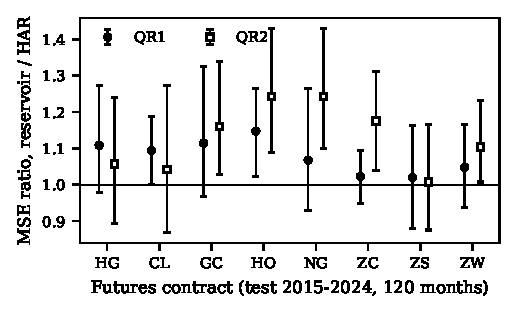
\includegraphics[width=\columnwidth]{figs/sanda3.pdf}
\caption{MSE ratio of the validation-selected reservoir to HAR for eight commodity futures, with 95\% stationary-bootstrap intervals. Values above one mean the reservoir is worse.}
\label{fig:transfer}
\end{figure}

\subsection{Execution on Quantum Hardware}
\label{sec:res-hw}
An exact implementation of $e^{-iH}$ for the all-to-all coupled Hamiltonian is deep. With second-order Suzuki--Trotter decomposition~\cite{suzuki1991}, the maximum error of a readout relative to the exact reservoir is 0.279 with one Trotter step, 0.076 with two, 0.020 with four, and 0.005 with eight (noiseless density-matrix simulation of 20 months). Compiled for an IBM Heron processor, the full three-lag circuit needs 972 two-qubit (CZ) gates with one step, 2016 with two, and 3907 with four. At the median CZ error of $2.45\times10^{-3}$, even one step leaves a rough success estimate of about 9\%. An accurate circuit is therefore out of reach of current hardware, and we ran the one-step circuit. Table~\ref{tab:trotter} summarizes the trade-off.

\begin{table}[t]
\caption{\textbf{Trotter accuracy and compiled cost of the QR1 circuit}}
\label{tab:trotter}
\setlength{\tabcolsep}{3pt}
\begin{tabular}{|c|c|c|c|c|c|}
\hline
Steps & Max error & Median error & CZ gates & Depth & Success est.\\
\hline
1 & 0.279 & 0.082 & 972 & 1748 & $9.2\times10^{-2}$\\
2 & 0.076 & 0.034 & 2016 & 3613 & $7.1\times10^{-3}$\\
4 & 0.020 & 0.009 & 3907 & 6962 & $6.9\times10^{-5}$\\
8 & 0.005 & 0.002 & -- & -- & --\\
\hline
\multicolumn{6}{p{240pt}}{Error: absolute difference of $\langle Z_q\rangle$ from the exact reservoir over 20 months, noiseless. Cost: full three-lag circuit compiled for an IBM Heron processor, with 14 mid-circuit resets. Success estimate: $(1-e)^{n_\mathrm{CZ}}$ with median CZ error $e=2.45\times10^{-3}$.}\\
\end{tabular}
\end{table}

We executed QR1 (validation-selected instance) on \emph{ibm\_marrakesh} with mid-circuit resets of the input qubits, no error mitigation, and Qiskit~\cite{qiskit2024}: a pilot of 60 months at 1000 shots, then all 813 months at 500 shots, using 168 s of processor time. In the 60-month pilot at 1000 shots, the hardware features already differed from the noiseless one-step circuit by 0.378 on average, and their median correlation with it was 0.83; the full run confirmed the pilot. The readout was trained on hardware features, so training and test features share the same noise.

Hardware features differ from the noiseless one-step circuit by 0.376 on average, against a shot-noise scale of 0.045, and their magnitude shrinks from 0.70 to 0.34 on average, as expected under depolarizing noise (Fig.~\ref{fig:hw}). Five of the seven input-qubit features keep a correlation of about 0.95 with their noiseless values. The three hidden qubits, which carry information across lags, behave differently: their mean values fall from about 0.86 to between 0.14 and 0.27, and their correlation with the noiseless values falls to between 0.13 and 0.29. Their variation is small even without noise (standard deviation about 0.03), so at 500 shots it is comparable to shot noise.

The forecasts follow. The test MSE is 0.1275 on hardware, against 0.1105 for the noiseless one-step circuit, 0.1064 for the exact reservoir, and 0.1156 for HAR. Hardware is significantly worse than all three after Holm correction (ratios 1.153, 1.198, and 1.103; $p_\mathrm{Holm}=0.010$, 0.005, and 0.042). We found no sign that hardware noise acted as a useful regularizer, as has been reported for another forecasting task~\cite{hamhoum2025}. This is one instance at one circuit depth without error mitigation.

\begin{figure}[t]
\centering
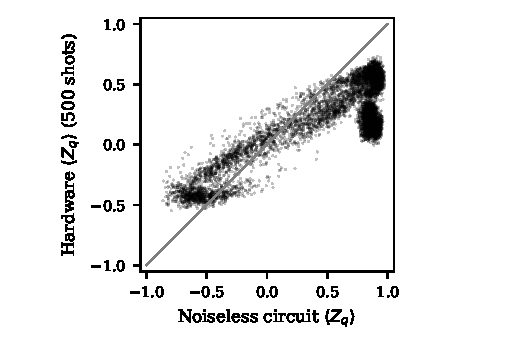
\includegraphics[width=\columnwidth]{figs/sanda5.pdf}
\caption{Readout features on IBM hardware (500 shots) against the same one-step circuit simulated without noise, for all 813 months and ten qubits. The cluster near a noiseless value of 0.9 that falls below the diagonal is mostly hidden-qubit features.}
\label{fig:hw}
\end{figure}

% ===========================================================================
\section{Discussion}
\label{sec:discussion}

\subsection{What Explains the Published Edge?}
The audit decomposes the published margin. Full-sample scaling contributes under 2\%. Choosing the reservoir instance by test performance places the reported model in the top decile of its family. Test-scored feature selection supplies inputs that suit the test period, and once inputs are chosen on validation data the edge over HAR disappears. A weak HAR benchmark (MSE 0.1476 instead of 0.1156) widens the reported gap further. What remains, the advantage of a validation-selected reservoir with published inputs, is not statistically distinguishable from HAR or from a tuned classical reservoir, and the sample could not have detected it reliably even without selection effects.

None of these steps is unusual in machine learning practice, and the paper is transparent that it reports best-performing configurations. The lesson is that best-of-$N$ reporting on the test period is not neutral even when applied to every model: it rewards whichever family has more variance across instances and choices, and it makes significance tests on the reported model invalid unless they account for the search~\cite{white2000,hansen2005,bailey2014}.

\subsection{Is There Anything Quantum Here?}
The proposition in Section~\ref{sec:res-surrogate} shows that, for this encoding, the reservoir computes a fixed multilinear trigonometric feature map whose coefficients depend on the couplings. The quantum dynamics choose which combinations of $\cos\pi x$ and $\sin\pi x$ terms appear, and on the authors' data this choice beats the uncoupled reservoir. But the same functional class is available classically: a second-order trigonometric regression reproduces the features almost exactly, and size-matched classical reservoirs and random features forecast as well. This agrees with surrogate theory~\cite{schuld2021,schreiber2023,sweke2025} and with benchmark evidence~\cite{fellner2026}. On hardware, the part of the computation that depends on deep entangling evolution, the hidden-qubit memory, is the part that noise removes.

\subsection{Recommendations for Quantum Forecasting Studies}
Our protocol suggests a short checklist for quantum, and indeed classical, forecasting claims (Table~\ref{tab:checklist}). Pre-registration with hashed files is cheap and makes the order of decisions verifiable.

\begin{table}[t]
\caption{\textbf{Checklist for quantum forecasting claims}}
\label{tab:checklist}
\setlength{\tabcolsep}{3pt}
\begin{tabular}{|p{110pt}|p{120pt}|}
\hline
Check & What this audit found without it\\
\hline
Select instances, hyperparameters and inputs on validation data; report all instances & published instances rank 5th and 7th of 100; test-scored selection reproduces the inputs\\
Use a standard, tuned benchmark & published HAR MSE 0.1476 against 0.1156 for a standard HAR\\
Add size-matched classical controls and an exact surrogate & tuned ESN and Trig2 not significantly worse\\
Correct for multiple comparisons and snooping (Holm, SPA, MCS) & SPA does not reject against HAR\\
Report the minimum detectable effect & 15--20\% needed; observed 7--8\%\\
Train hardware readouts on hardware features & hardware features lose the hidden-qubit memory\\
\hline
\end{tabular}
\end{table}

\subsection{Threats to Validity}
\emph{Internal validity.} Our implementation could differ from the authors' in ways that matter only for instances or inputs they did not publish. The reproduction to $1.2\times10^{-6}$ for both published designs, and of AR(3) and both QLIKE values, makes this unlikely. \emph{Construct validity.} We judge the claim by forecast losses on log RV and variance, as the original paper does; other uses of a volatility forecast, such as risk limits or option pricing, could weigh errors differently. \emph{Statistical conclusion validity.} With 245 test months, the tests have low power for realistic gains (Section~\ref{sec:res-power}), so a non-significant result is not evidence of equality; this is why we also report point ratios, intervals and the comparison with size-matched controls. \emph{External validity.} The audit concerns one claim, and the commodity transfer and hardware run test the design, not quantum reservoirs in general.

\subsection{Limitations}
This audit examines one published study, one reservoir family, and one encoding. The trigonometric description depends on fresh re-encoding of each input value; reservoirs with feedback or repeated encoding of the same value can produce higher frequencies and may behave differently. The commodity transfer uses 120 test months and, as Section~\ref{sec:res-power} shows, cannot confirm small gains. The hardware experiment uses one instance, one Trotter depth, and no error mitigation. One change to the controls was made after results were seen (Appendix~\ref{app:deviations}); it changed no decision. Finally, the authors' repository carries no licence, so our replication package links to their data at a fixed commit instead of redistributing it.

% ===========================================================================
\section{Conclusion}
\label{sec:conclusion}
A published claim that quantum reservoir computing forecasts realized volatility better than classical methods reproduces exactly but does not survive honest evaluation. The advantage depends on choices that coincide with the test period, is matched by classical models of the same size, falls below what the sample can detect, does not transfer to eight commodity markets, and is lost on current hardware. The reservoir itself is, by proof and in practice, a low-order trigonometric feature map. We hope the audit protocol and its checklist help quantum machine learning for finance build claims that last. Future work should test reservoirs with feedback or repeated encoding of the same input, which fall outside the trigonometric description, and error-mitigated hardware runs at greater circuit depth.

\section*{Data and Code Availability}
Code, registrations with their hashes, and all derived results: \url{https://github.com/Janindu2204/qrc-volatility-audit}, archived as release v1.0 (commit 0a315b6) on Zenodo, doi: 10.5281/zenodo.24398016. The data and couplings of Li \emph{et al.} are available from their repository at commit d2e9b0aa (\url{https://github.com/LeeQY1996/Quantum-Reservoir-computing-for-Realized-Volatility-Forecasting}). Commodity, VIX, and dollar-index data were downloaded from the Yahoo Finance chart interface with the fetch script in the repository. IBM job identifiers: dbr91k7v5hds73dhcq30 (pilot) and dbr924mjjaos73aik6u0 (full run).

\section*{Competing Interests}
The authors declare no competing interests.

\appendices
\section{Proof of the Proposition}
\label{app:proof}
Fix a forecast month and write $x_{k,v}$ for input $v$ at lag $k$. The input qubit for $(k,v)$ is prepared in $|\psi\rangle=\cos(\pi x/2)|0\rangle+\sin(\pi x/2)|1\rangle$ with $x=x_{k,v}$, so its density matrix is
\begin{equation}
\rho(x)=\tfrac12\left(I+\cos(\pi x)\,Z+\sin(\pi x)\,X\right).
\label{eq:rho}
\end{equation}
In matrix form its diagonal entries are $(1\pm\cos\pi x)/2$ and its off-diagonal entries are $(\sin\pi x)/2$, so each entry is affine in $(1,\cos\pi x,\sin\pi x)$. The full computation is a composition of unitary evolutions, partial traces over discarded input qubits, and tensoring with freshly prepared qubits. Each of these maps is linear in every tensor factor it acts on, and each value $x_{k,v}$ enters through exactly one tensor factor, $\rho(x_{k,v})$, which is never copied. Hence the final state is a multilinear function of the 21 matrices $\rho(x_{k,v})$, and so is $\langle Z_q\rangle=\mathrm{Tr}(Z_q\rho_\mathrm{final})$. Substituting \eqref{eq:rho}, every readout is a linear combination of products $\prod_{k,v} g_{k,v}(x_{k,v})$ with $g_{k,v}\in\{1,\cos\pi x,\sin\pi x\}$, which is the claim. The same argument applies to the readout halfway through the last evolution (QR2), to any couplings, and to any fixed Hamiltonian. The order-$r$ truncation keeps products with at most $r$ non-constant factors; for 21 inputs it has 43 terms at $r=1$ and 883 at $r=2$.

\section{Deviations From the Registrations}
\label{app:deviations}
\emph{Gain concentration (post hoc).} The analysis of Section~\ref{sec:res-concentration} was added after all registered tests were reported. It uses only the saved Test 2 forecasts and is descriptive.

\emph{Addendum A1 (post hoc).} The registered readout has no intercept. Quantum features have non-zero means that act as an intercept, but the RandTrig and RFF controls are close to zero-mean and could not fit the level of the target; on the commodity data their median test MSE was two to three times that of HAR. After seeing the Test 7 results we rebuilt both controls as $p-1$ random features plus a constant column, keeping $p$ readout columns and all seeds and selection rules. This changed no registered decision. On the authors' data the claim still fails; on commodities the edge count stays at zero of eight for both designs; and the number of significant results in favor of the reservoir in Test 7 falls from 20 to 5, showing that most were artifacts of the broken controls. The registered results are reported alongside in the replication package.

\emph{Supplementary analyses.} The finer power grid (Table~\ref{tab:power}, Fig.~\ref{fig:power}) supplements the registered grid and agrees with it. No predictions were recorded before the runs.

\section*{Acknowledgment}
The authors thank Li, Mukhopadhyay, Bayat, and Habibnia for releasing their code, data, and couplings, which made this audit possible.

The authors used Claude (Anthropic), through the Claude Code tool (November 2026), as an assistant throughout this work. It drafted the analysis and simulation code, the pre-registration files, the figure scripts, and first drafts of all sections of the manuscript, and it assisted with literature searches and with checking references against Crossref and arXiv. All study design decisions, registrations, and interpretations were reviewed and approved by the authors. The authors reviewed all code, results, references, and text, and take full responsibility for the content of this article.

\begin{thebibliography}{00}

\bibitem{bowles2024}J. Bowles, S. Ahmed, and M. Schuld, ``Better than classical? The subtle art of benchmarking quantum machine learning models,'' 2024, \emph{arXiv:2403.07059 [quant-ph]}.

\bibitem{schuld2021}M. Schuld, R. Sweke, and J. J. Meyer, ``Effect of data encoding on the expressive power of variational quantum-machine-learning models,'' \emph{Phys. Rev. A}, vol. 103, no. 3, 2021, Art. no. 032430, doi: 10.1103/PhysRevA.103.032430.

\bibitem{schreiber2023}F. J. Schreiber, J. Eisert, and J. J. Meyer, ``Classical surrogates for quantum learning models,'' \emph{Phys. Rev. Lett.}, vol. 131, no. 10, 2023, Art. no. 100803, doi: 10.1103/PhysRevLett.131.100803.

\bibitem{sweke2025}R. Sweke \emph{et al.}, ``Potential and limitations of random Fourier features for dequantizing quantum machine learning,'' \emph{Quantum}, vol. 9, 2025, Art. no. 1640, doi: 10.22331/q-2025-02-20-1640.

\bibitem{white2000}H. White, ``A reality check for data snooping,'' \emph{Econometrica}, vol. 68, no. 5, pp. 1097--1126, 2000, doi: 10.1111/1468-0262.00152.

\bibitem{hansen2005}P. R. Hansen, ``A test for superior predictive ability,'' \emph{J. Bus. Econ. Statist.}, vol. 23, no. 4, pp. 365--380, 2005, doi: 10.1198/073500105000000063.

\bibitem{bailey2014}D. H. Bailey, J. M. Borwein, M. L\'opez de Prado, and Q. J. Zhu, ``Pseudo-mathematics and financial charlatanism: The effects of backtest overfitting on out-of-sample performance,'' \emph{Notices Amer. Math. Soc.}, vol. 61, no. 5, pp. 458--471, 2014, doi: 10.1090/noti1105.

\bibitem{kapoor2023}S. Kapoor and A. Narayanan, ``Leakage and the reproducibility crisis in machine-learning-based science,'' \emph{Patterns}, vol. 4, no. 9, 2023, Art. no. 100804, doi: 10.1016/j.patter.2023.100804.

\bibitem{fellner2026}T. Fellner, D. A. Kreplin, S. Tovey, and C. Holm, ``Quantum vs. classical: A comprehensive benchmark study for predicting time series with variational quantum machine learning,'' \emph{Mach. Learn.: Sci. Technol.}, vol. 7, no. 1, 2026, Art. no. 010501, doi: 10.1088/2632-2153/ae365f.

\bibitem{gillani2026}S. A. Gillani, M. S. A. Baig, S. M. Shah, A. Ali, and H. Siddiqui, ``How quantum is the advantage? A fair, calibration- and noise-aware benchmark and attribution audit of quantum machine learning for network intrusion detection,'' 2026, \emph{arXiv:2608.18155 [quant-ph]}.

\bibitem{li2026}Q. Li, C. Mukhopadhyay, A. Bayat, and A. Habibnia, ``Quantum reservoir computing for realized volatility forecasting,'' \emph{Phys. Rev. Res.}, vol. 8, no. 2, 2026, Art. no. 023028, doi: 10.1103/rbj7-4wnq.

\bibitem{jaeger2001}H. Jaeger, ``The `echo state' approach to analysing and training recurrent neural networks,'' German Nat. Res. Center Inf. Technol., Sankt Augustin, Germany, GMD Rep. 148, 2001.

\bibitem{fujii2017}K. Fujii and K. Nakajima, ``Harnessing disordered-ensemble quantum dynamics for machine learning,'' \emph{Phys. Rev. Appl.}, vol. 8, no. 2, 2017, Art. no. 024030, doi: 10.1103/PhysRevApplied.8.024030.

\bibitem{mujal2021}P. Mujal \emph{et al.}, ``Opportunities in quantum reservoir computing and extreme learning machines,'' \emph{Adv. Quantum Technol.}, vol. 4, no. 8, 2021, Art. no. 2100027, doi: 10.1002/qute.202100027.

\bibitem{martinezpena2023}R. Mart\'inez-Pe\~na and J.-P. Ortega, ``Quantum reservoir computing in finite dimensions,'' \emph{Phys. Rev. E}, vol. 107, no. 3, 2023, Art. no. 035306, doi: 10.1103/PhysRevE.107.035306.

\bibitem{rahimi2007}A. Rahimi and B. Recht, ``Random features for large-scale kernel machines,'' in \emph{Proc. Adv. Neural Inf. Process. Syst. (NIPS)}, vol. 20, 2007, pp. 1177--1184.

\bibitem{hernicht2026}P. Hernicht \emph{et al.}, ``Enhancing the scalability of classical surrogates for real-world quantum machine learning applications,'' \emph{Quantum Mach. Intell.}, vol. 8, no. 2, 2026, Art. no. 83, doi: 10.1007/s42484-026-00420-6.

\bibitem{tudisco2024}A. Tudisco \emph{et al.}, ``Evaluating the computational advantages of the variational quantum circuit model in financial fraud detection,'' \emph{IEEE Access}, vol. 12, pp. 102918--102940, 2024, doi: 10.1109/ACCESS.2024.3432312.

\bibitem{pandey2026}T. Pandey, ``When classical baselines are tuned as carefully as the quantum model, does quantum reservoir computing still win?'' 2026, \emph{arXiv:2607.09905 [quant-ph]}.

\bibitem{shen2026}J. Shen, ``Quantum kernels and the cross-section of stock returns: Anatomy of a vanishing advantage,'' 2026, \emph{arXiv:2607.20168 [q-fin.PR]}.

\bibitem{islam2026}M. R. Islam, ``Benchmarking quantum machine learning for power-system attack detection: Evaluation choices decide the outcome before the models do,'' 2026, \emph{arXiv:2608.15617 [cs.LG]}.

\bibitem{maheshwari2026}D. Maheshwari, G. Hellstern, M. Zaefferer, M. Braun, and T. D\"ohler, ``Quantum recurrent architectures for financial time series prediction,'' 2026, \emph{arXiv:2611.15298 [quant-ph]}.

\bibitem{andersen2003}T. G. Andersen, T. Bollerslev, F. X. Diebold, and P. Labys, ``Modeling and forecasting realized volatility,'' \emph{Econometrica}, vol. 71, no. 2, pp. 579--625, 2003, doi: 10.1111/1468-0262.00418.

\bibitem{corsi2009}F. Corsi, ``A simple approximate long-memory model of realized volatility,'' \emph{J. Financial Econometrics}, vol. 7, no. 2, pp. 174--196, 2009, doi: 10.1093/jjfinec/nbp001.

\bibitem{diebold1995}F. X. Diebold and R. S. Mariano, ``Comparing predictive accuracy,'' \emph{J. Bus. Econ. Statist.}, vol. 13, no. 3, pp. 253--263, 1995, doi: 10.1080/07350015.1995.10524599.

\bibitem{newey1987}W. K. Newey and K. D. West, ``A simple, positive semi-definite, heteroskedasticity and autocorrelation consistent covariance matrix,'' \emph{Econometrica}, vol. 55, no. 3, pp. 703--708, 1987, doi: 10.2307/1913610.

\bibitem{hansen2011}P. R. Hansen, A. Lunde, and J. M. Nason, ``The model confidence set,'' \emph{Econometrica}, vol. 79, no. 2, pp. 453--497, 2011, doi: 10.3982/ECTA5771.

\bibitem{patton2011}A. J. Patton, ``Volatility forecast comparison using imperfect volatility proxies,'' \emph{J. Econometrics}, vol. 160, no. 1, pp. 246--256, 2011, doi: 10.1016/j.jeconom.2010.03.034.

\bibitem{welch2008}I. Welch and A. Goyal, ``A comprehensive look at the empirical performance of equity premium prediction,'' \emph{Rev. Financial Stud.}, vol. 21, no. 4, pp. 1455--1508, 2008, doi: 10.1093/rfs/hhm014.

\bibitem{politis1994}D. N. Politis and J. P. Romano, ``The stationary bootstrap,'' \emph{J. Amer. Statist. Assoc.}, vol. 89, no. 428, pp. 1303--1313, 1994, doi: 10.1080/01621459.1994.10476870.

\bibitem{holm1979}S. Holm, ``A simple sequentially rejective multiple test procedure,'' \emph{Scand. J. Statist.}, vol. 6, no. 2, pp. 65--70, 1979, doi: 10.2307/4615733.

\bibitem{suzuki1991}M. Suzuki, ``General theory of fractal path integrals with applications to many-body theories and statistical physics,'' \emph{J. Math. Phys.}, vol. 32, no. 2, pp. 400--407, 1991, doi: 10.1063/1.529425.

\bibitem{qiskit2024}A. Javadi-Abhari \emph{et al.}, ``Quantum computing with Qiskit,'' 2024, \emph{arXiv:2405.08810 [quant-ph]}.

\bibitem{hamhoum2025}W. Hamhoum, S. Cherkaoui, J.-F. Laprade, O. Ahmad, and S. Wang, ``Multivariate time series forecasting with gate-based quantum reservoir computing on NISQ hardware,'' 2025, \emph{arXiv:2510.13634 [cs.LG]}.

\end{thebibliography}

% [TODO] Replace IEEEbiographynophoto by IEEEbiography with the photo file once it is available:
% \begin{IEEEbiography}[{\includegraphics[width=1in,height=1.25in,clip,keepaspectratio]{PHOTO_FILE}}]{...}
\begin{IEEEbiographynophoto}{Sandanayakage Janindu Indira Sandanayaka}
is currently pursuing the B.Sc. degree in computer science at the Informatics Institute of Technology, Colombo, Sri Lanka, in collaboration with the University of Westminster, London, U.K., with expected graduation in 2027. Research interests include quantum machine learning, financial time-series forecasting, and the reproducible evaluation of machine learning claims.
\end{IEEEbiographynophoto}


\EOD

\end{document}
